%Talk given virtually to Mac Hyman and friends, November 15, 2021
\documentclass[10pt,compress,xcolor={usenames,dvipsnames},aspectratio=169]{beamer}
%\documentclass[xcolor={usenames,dvipsnames},aspectratio=169]{beamer} %slides and 
%notes
\usepackage[T1]{fontenc}
\usepackage{tgadventor} %Font found at https://tug.org/FontCatalogue/
%\usepackage{newpxtext}
\usepackage[euler-digits,euler-hat-accent]{eulervm}

\usepackage{amsmath,
	amssymb,
	datetime,
	mathtools,
	bbm,
	%mathabx,
	array,
	booktabs,
	xspace,
	multirow,
	calc,
	colortbl,
	siunitx,
 	graphicx}
\usepackage[usenames]{xcolor}
\usepackage[giveninits=false,backend=biber,style=nature, maxcitenames =10, mincitenames=9]{biblatex}
\addbibresource{FJHown23.bib}
\addbibresource{FJH23.bib}
\usepackage{media9}
\usepackage[autolinebreaks]{mcode}
\usepackage[overlay,absolute]{textpos}
\usepackage[tikz]{mdframed}


\usetheme{FJHSlimNoFoot169}
\setlength{\parskip}{2ex}
\setlength{\arraycolsep}{0.5ex}
\newcommand{\squeezeeqspace}[1]{%
	\setlength{\abovedisplayskip}{#1}%
	\setlength{\belowdisplayskip}{#1}%
}



\usepackage{algpseudocode}
\usepackage{algorithm, algorithmicx}
\algnewcommand\algorithmicproblem{\textbf{Problem:}}
\algnewcommand\PROB{\item[\algorithmicproblem]}
\algnewcommand\algorithmicparam{\textbf{Parameters:}}
\algnewcommand\PARAM{\item[\algorithmicparam]}
\algnewcommand\algorithmicinput{\textbf{Input:}}
\algnewcommand\INPUT{\item[\algorithmicinput]}
\algnewcommand\RETURN{\State \textbf{Return }}



\DeclareMathOperator{\BUMP}{bump}
\DeclareMathOperator{\TRAP}{TRAP}
\DeclareMathOperator{\COST}{COST}
\DeclareMathOperator{\STOP}{STOP}
\DeclareMathOperator{\DATA}{ACC}
\DeclareMathOperator{\SOL}{SOL}
\DeclareMathOperator{\OUT}{OUT}
\DeclareMathOperator{\CRIT}{CRIT}
\DeclareMathOperator{\APP}{APP}
\DeclareMathOperator{\ERR}{ERR}
\DeclareMathOperator{\AVG}{AVG}
\DeclareMathOperator{\INT}{INT}
\DeclareMathOperator{\LIN}{LINEAR}
\DeclareMathOperator{\BAD}{BAD}
%\DeclareMathOperator{\opt}{opt}
\newcommand{\dataN}{\bigl(\hf(\vk_i)\bigr)_{i=1}^n}
\newcommand{\dataNj}{\bigl(\hf(\vk_i)\bigr)_{i=1}^{n_j}}
\newcommand{\dataNjd}{\bigl(\hf(\vk_i)\bigr)_{i=1}^{n_{j^\dagger}}}
\newcommand{\ERRN}{\ERR\bigl(\dataN,n\bigr)}
\newcommand{\otod}{\ensuremath{1\mkern-4mu : \mkern-2mu d}}
\newcommand{\ttrue}{\textup{true}}
\newcommand{\tfalse}{\textup{false}}
\newcommand{\tolabs}{\varepsilon_{\textup{a}}}
\newcommand{\tolrel}{\varepsilon_{\textup{r}}}


%\DeclareMathOperator{\app}{app}

\providecommand{\HickernellFJ}{H.\xspace}


\renewcommand{\OffTitleLength}{-7ex}
\setlength{\FJHThankYouMessageOffset}{-8ex}
\title{Complexity of Numerical Problems}
\author[]{GAIL/QMCPy/GAAPy Group}
\institute{Department of Applied Mathematics \qquad
	Center for Interdisciplinary Scientific Computation \\
	Illinois Institute of Technology \qquad
	\href{mailto:hickernell@iit.edu}{\url{hickernell@iit.edu}} \qquad
	\href{http://mypages.iit.edu/~hickernell}{\url{mypages.iit.edu/~hickernell}}}

\thanksnote{}
	
\date[]{ revised \today}

\input FJHDef.tex



\begin{document}
	\everymath{\displaystyle}

\frame{\titlepage}

%%%%%%%%%%%%%%%%%%%%%%%%%%%%%%%%%%%%%%%%%%
%%%%%%%%%%%%%%%%%%%%%%%%%%%%%%%%%%%%%%%%%%

\part{Problems and Algorithms}
\section{Problems}
%%%%%%%%%%%%%%%%%%%%%%%%%%%%%%%%%%%%%%%%%%
%%%%%%%%%%%%%%%%%%%%%%%%%%%%%%%%%%%%%%%%%%

\begin{frame}{Mathematical Problems}

\vspace{-5ex}
Define a (continuous) \alert{mathematical problem} as
\begin{align*}
    \cf & = \text{set of input functions defined on the domain } \Omega\\
    \cg & = \text{set of possible solutions} \\
    \SOL :\cf \to \cg &= \text{a solution operator}
\end{align*}
Examples include integration and root-finding
\begin{align*}
   \cf &=  C[0,1] & \cf &= C[0,1]\\
    \cg & = \reals &  \cg &= \text{set of all closed subsets of } [0,1]\\
    \SOL(f) &= \int_0^1 f(x) \, \dif x & \SOL(f) & = f^{-1}(0)
\end{align*}
\end{frame}

\begin{frame}{Existence and Analytic Solutions}
\squeezeeqspace{6pt}

\vspace{-4ex}
For mathematical problems, $\SOL:\cf \to \cg$, one may prove \alert{existence}
	\begin{align*}
   		\cf &=  C[0,1] & \cf &= C[0,1]\\
		\cg & = \reals &  \cg &= \text{set of all closed subsets of } [0,1]\\
		\SOL(f) & \text{ exists} & \SOL(f) & \text{ exists, even if it is the null set}
	\intertext{\uncover<2->{One may construct \alert{analytical solutions} via symbolic computation \cite{Coh03a} for some \alert{smaller $\cf$} than that which admits existence:}}
	\multispan2{\uncover<2->{$\SOL(x \mapsto x \exp(-2x)) = \frac {1 - 3 \exp(-2)}4$}} & 
			\multispan2{\uncover<2->{$\SOL(x \mapsto 4 x^2 - 6x + 1)  = \left \{ \frac {3 \pm \sqrt{5}}{4}  \right\}$}}
	\intertext{\uncover<3->{Analytical solutions, $\SOL(f)$ may \alert{not be available} if $f$ is too complex. Then we need \alert{numerical solutions}}}
			\multispan2{\uncover<3->{\hfil$\SOL(\text{black-box}) =?$\hfil}} &
            \multispan2{\uncover<3->{\hfil$\SOL(\text{black-box}) =?$\hfil}}
	\end{align*}
\uncover<3->{We discover information about input function $\text{black-box}(\cdot)$---apart from its membership in $\cf$---through  \alert {data operators} applied to  $\text{black-box}(\cdot)$.}
	
\end{frame}

\begin{frame}{Numerical Problems}

\vspace{-5ex}
For mathematical problem $\SOL:\cf \to \cg$, numerical solution, $\OUT$, should be be close to true solution, $\SOL(f)$, according to an error criterion, $\CRIT$, and tolerance, $\veps$:
\begin{align*}
    \OUT & = \text{numerical solution} \in \cg \\
    \veps & = \text{scalar or vector of error tolerances} \in \ce \subseteq [0,\infty)^s\\
    \CRIT: \cg \times \cg \times \ce \to \{\ttrue, \tfalse\}& = \text{error criterion} \\
\intertext{\alert{Acceptable numerical solutions} satisfy $\CRIT(\OUT,\SOL(f),\veps) = \ttrue$. \endgraf
\uncover<2->{In addition to knowledge about $f$ based on the definition of $\cf$, the algorithm constructing the numerical solution \alert{samples} $f$, e.g., by generating function values or  derivative values:}}
    \uncover<2->{\Lambda: \cf \to \reals^t} &\uncover<2->{= \text{set of allowable \alert{data operators}}}
\end{align*}
\uncover<2->{A \alert{numerical problem} is described by the ordered triple $(\SOL, \CRIT, \Lambda)$.}

\end{frame}

\begin{frame}{Choosing $\cf$ for Numerical Problems}
	\vspace{-5ex}
	The set of input functions, $\cf$, chosen to prove \alert{existence} or to construct \alert{analytical solutions} are different from the $\cf$ for numerical problems.  These latter $\cf$ should be
	\begin{itemize}
		\item Often a \alert{ball} or \alert{cone}, usually not a vector space
		\item Small enough so that an algorithm \alert{exists} to solve $(\SOL,\CRIT,\Lambda)$
		\item Small enough to admit algorithms with the desired  \alert{computational cost}
		\item Large enough to include the input functions  expected in \alert{practice}
	\end{itemize}
Think \alert{Goldilocks}
	
\end{frame}


\section{Algorithms}


\begin{frame}{Data}
	
	\vspace{-5ex}
	Now we discuss \alert{algorithms} to solve numerical problems.
	$(\SOL, \CRIT, \Lambda)$ is assumed fixed.
	
	Algorithms work with function data that takes the form
	\[
	\mZ_n 
	= \begin{pmatrix} \vL_n & \mY_n \end{pmatrix}
	=  \begin{pmatrix} L_{1} & L_{1}(f) \\ \vdots & \vdots \\ L_{n} & L_{n}(f) \end{pmatrix} 
	\in \Lambda^n \times \reals^{n\times t}
	\]
	$\vL_n$ is the \alert{design}.  Sometimes we drop the subscript $n$.
	
	\uncover<2->{When the set of possible data operators, $\Lambda$, consists of function evaluations, then we may represent the design by the data sites, $\mX_n = (\vx_1, \ldots, \vx_n)^T \in \Omega^n \subseteq \reals^{n \times d}$:
	\[
	\mZ_{n} = \begin{pmatrix} \mX & f(\mX_{n}) \end{pmatrix} \in  \reals^{n \times (d+t)}
	\]}
	
	
\end{frame}


\begin{frame}{Stopping Criteria}

\vspace{-5ex}
The \alert{data based} stopping criterion
\[
\STOP:  \ce  \times \cup_{n \in \natzero} (\Lambda^n \times \reals^{n\times t} ) \to \cg \times 2^\cg \times \{\ttrue, \tfalse \}
\]
determines whether there exists an output, $\OUT$, satisfying the error criterion, $\CRIT(\OUT,\SOL(f),\veps)$.   

Given the function data $\mZ =\begin{pmatrix}\vL & \mY\end{pmatrix}$,  construct 
\[
\cg(\mZ) \supseteq \{\SOL(f) :   f \in \cf, \ \vL(f) = \mY   \} = \text{ set of solutions consistent with function data}
\]
The data based stopping criterion is defined by
\[
\STOP(\veps,\mZ) = \begin{cases} 
	(\OUT,\cg(\mZ), \ttrue), & 
	\exists \OUT \text{ such that } \CRIT(\OUT,g,\veps) = \ttrue \quad \forall g \in \cg(\mZ), \\
	(\OUT,\cg(\mZ),\tfalse), & \text{otherwise ($\OUT$ arbitrary, may be ``best'' so far)}
	\end{cases}
\]

\end{frame}



\begin{frame}{Data Accumulation}

\vspace{-4ex}

Function data $\mZ =\begin{pmatrix}\vL & \mY\end{pmatrix}$ is accumulated iteratively via the \alert{data accumulator},
\[
\DATA: \cf \times  \ce \times\cup_{n \in \natzero} (\Lambda^n \times \reals^{n\times t} ) \times 2^\cg\to  \cup_{n \in \naturals} (\Lambda^n \times \reals^{n\times t})
\]
Let $\mZ_0 = (\emptyset, \emptyset)$ and $\mZ_n \in \Lambda^n \times \reals^{n\times t}$.  Then,
\begin{gather*}
\DATA(f,\veps, \mZ_0, \cg) = 
\begin{pmatrix} L_{1} & L_{1}(f) \\ \vdots & \vdots \\ L_{n_1} & L_{n_1}(f) \end{pmatrix} 
= \begin{pmatrix}
	\vL_{n_1} & \mY_{n_1}
\end{pmatrix}
= \mZ_{n_1}, \\ 
\DATA(f, \veps,\mZ_{n_1}, \cg(\mZ_{n_1})) = 
\begin{pmatrix}\mZ_{n_1} \\ \begin{pmatrix} L_{n_1+1} & L_{n_1+1}(f) \\ \vdots & \vdots \\ L_{n_2} & L_{n_2}(f) \end{pmatrix}  \end{pmatrix} 
= \begin{pmatrix}
	\vL_{n_2} & \mY_{n_2}
\end{pmatrix}
= \mZ_{n_2}, \quad \ldots
\end{gather*}
where $0 < n_1 < n_2 < \cdots$.  \alert{Adaptive} designs, $\vL_{n_{\ell+1}}$, depend  on $ \cg(\mZ_{n_\ell})$.

\end{frame}

\section{Examples}
\begin{frame}[label = traprule]{Trapezpoidal Rule Integration \hyperlink{difference}{\beamergotobutton{Why success?}}}

\vspace{-2ex}
For the integration problem above with a \alert{compound error criterion}
\vspace{-1ex}
\begin{gather*}
	\cf = \{f \in C^1[0,1] : \norm[2]{f''} \le 1\}, \qquad 
	\cg  = \reals,  \qquad
	\SOL(f) = \int_0^1 f(x) \, \dif x  \\
	\CRIT(\OUT, \SOL(f),(\tolabs, \tolrel))  = \begin{cases} \ttrue, & \abs{\SOL(f) - \OUT} \le \max(\tolabs,\tolrel \abs{\SOL(f)}), \\
		\tfalse, & \text{otherwise}, 
		\end{cases} \\
	 (\tolabs,\tolrel) \in (0,\infty) \times [0,1), \qquad
	 \Lambda  = \{L :  L(f) = f(x) \text{ for some } x \in [0,1]\} = \text{function evaluations}
\end{gather*}
\uncover<2->{Use a \alert{nonadaptive} data accumulator to construct $\mZ = \begin{pmatrix} \mX & f(\mX) \end{pmatrix}$:
\vspace{-1ex}
\begin{gather*}
\mZ_2 = \DATA(f,\veps,\mZ_{0},\cg)  = \begin{pmatrix} 0 & f(0) \\ 1 & f(1) \end{pmatrix},  \quad
\mZ_3 = \DATA(f,\veps,\mZ_{2},\cg(\mZ_{2})) = \begin{pmatrix} 0 & f(0) \\ 1 & f(1) \\ 1/2 & f(1/2)\end{pmatrix}, \\
	\mZ_{n+1} =  \begin{pmatrix} \mX_{n+1} & f(\mX_{n+1}) \end{pmatrix} = \DATA(f,\veps,\mZ_{n/2+1},\cg(\mZ_{n/2+1})) = \begin{pmatrix} \mX_{n/2+1} & f(\mX_{n/2+1}) \\ 1/n& f(1/n) \\ 3/n & f(3/n) \\ \vdots & \vdots \\ 1 - 1/n & f(1 - 1/n)\end{pmatrix}  \text{ for } \log_2(n) \in \naturals
\end{gather*}}

\end{frame}

\begin{frame}{Trapezpoidal Rule Integration cont'd}

\vspace{-6ex}
\begin{gather*}
	\cf = \{f \in C^1[0,1] : \norm[2]{f''} \le 1\}, \quad 
	\cg  = \reals,  \quad
	\SOL(f) = \int_0^1 f(x) \, \dif x, \quad   \Lambda = \text{function evaluations} \\
	\CRIT(\OUT, \SOL(f),(\tolabs, \tolrel))  = \begin{cases} \ttrue, & \abs{\SOL(f) - \OUT} \le \max(\tolabs,\tolrel \abs{\SOL(f)}), \\
		\tfalse, & \text{otherwise},
		\end{cases} \\
		\text{\alert{trapezoidal rule}: } 
		\TRAP(\mZ_2) = \frac 1{2} \bigl( f(0) + f(1) \bigr), \\  
		\TRAP(\mZ_{n+1}) = \frac {1}{2}\TRAP(\mZ_{n/2+1}) + \frac 1{n} \left( f(1/n) + f(3/n) \cdots + f(1 -1/n) \right)  \quad \log_2(n) \in \naturals,\\
		\cg(\mZ_{n+1}) = \{I \in \reals : \abs{I - \TRAP(\mZ_{n+1})} \le \ERR_n\},  \quad \ERR_n =  1/??n^2, \qquad \text{\cite[(7.??)]{BraPet11a}}, \\ 
		\OUT = \TRAP(\mZ_{n+1}) + \frac 12 \left[\max(\tolabs,\tolrel\abs{\TRAP(\mZ_{n+1})- \ERR_n}) - \max(\tolabs,\tolrel \abs{\TRAP(\mZ_{n+1}) +\ERR_n}) \right] \\
		\text{minimizes }  \max_{I \in \cg(\mZ_{n+1})} \bigl[ \abs{I - \OUT} - \max(\tolabs,\tolrel \abs{I}) 
		\bigr ] \qquad \OUT \text{ may differ from } \TRAP(\mZ_{n+1}) \\
	\STOP(\veps,\mZ_{n+1}) 
	= \begin{cases} 
		(\OUT,\cg(\mZ_{n+1}), \ttrue), & 
		2\ERR_n \le  \max(\tolabs,\tolrel\abs{\TRAP(\mZ_{n+1})- \ERR_n}) \\
		& \qquad + \max(\tolabs,\tolrel\abs{\TRAP(\mZ_{n+1}) +\ERR_n}), \\
		(\OUT,\cg(\mZ_{n+1}),\tfalse), & \text{otherwise}.
	\end{cases}
\end{gather*}

\end{frame}


\begin{frame}{Algorithm}
	
\vspace{-2ex}
\begin{algorithm}[H]
	\renewcommand{\thealgorithm}{}
	\caption{General Algorithm Pattern}
	\begin{algorithmic}
		\PROB $(\SOL, \CRIT,\Lambda)$
		\INPUT black-box function, $f$;  error tolerance, $\veps$
		
		\Ensure  $\CRIT(\OUT,\SOL(f),\veps) = \ttrue$
		
		\State $\mZ \leftarrow (\emptyset, \emptyset)$
				
		\Repeat 
		
		\State $\mZ \leftarrow \DATA(f,\mZ)$

		\State $(\OUT,\text{done}) \leftarrow \STOP(\veps,\mZ)$
				
		\Until{$\text{done} = \ttrue$}
		
		\State $n  \leftarrow \text{\# rows in } \mZ$
		
		\RETURN $\OUT$, $n$
	\end{algorithmic}
\end{algorithm}	
\end{frame}


\section{No Algorithms Exist}

\begin{frame}{A Numerical Problem May Have No Possible Algorithm}
\squeezeeqspace{6pt}
	\vspace{-2ex}
{\small\begin{theorem} Suppose that
	\begin{gather*}
		\cg \text{ is a normed space}\qquad \SOL \text{ is homogeneous} \qquad \Lambda \subseteq \text{all homogeneous functionals}\\
		\cf = \text{cone of input functions with the property that for all $\vL_n \in \Lambda^n$ there exists an $h \in \cf$ } \\
		 \text{with $\vL_n(h) = \vzero_n$ and $\norm[\cg]{\SOL(h)} > 0$, \qquad
			e.g.,  $\SOL(\cf)$ is $\infty$-dimensional vector space} \\
		\CRIT(\OUT,\SOL,(\tolabs,\tolrel))  = \ttrue \iff  \norm[\cg]{\SOL(f) - \OUT} \le \max(\tolabs,\tolrel \norm[\cg]{\SOL(f)}), \\
		0 < \tolabs < \infty, \ 0 \le \tolrel < 1
	\end{gather*}
Then \alert{no algorithm} can solve $(\SOL, \CRIT, \Lambda)$.
\end{theorem}}
\uncover<2->{\small\begin{proof}\squeezeeqspace{2pt}
\only<2>{Suppose such an algorithm exists.  Fix $(\tolabs,\tolrel)$.  Let $f=0$ be the input.  After $n$ function values the algorithm terminates with the data matrix $\begin{pmatrix} \vL_n &\vzero_n \end{pmatrix}$ and numerical solution $\OUT$.  There exists some $h \in \cf$  with $\norm[\cg]{\SOL(h)} > 0$ and $\vL_n(h) = \vzero_n$.  So for any $c > 0$, the input $\pm ch$ causes the algorithm to terminate with the  \alert{same} $\OUT$.  Thus, \ldots \let\qedsymbol\relax}\only<3>{\vspace{-2ex}
\begin{align*}
	\max(\tolabs,\tolrel c\norm[\cg]{\SOL(h)}) &
	\ge \frac 12 \bigl[ \norm[\cg]{\SOL(ch) - \OUT} + \norm[\cg]{\SOL(-ch) - \OUT} \bigr]\\
	&= \frac 12 \bigl[ \norm[\cg]{c\SOL(h) - \OUT} + \norm[\cg]{c\SOL(h) + \OUT} \bigr]
	\ge  c \norm[\cg]{\SOL(h) } \quad \forall c
\end{align*}
which is impossible.  (Remember Goldilocks; $\cf$ is too big.)}
\end{proof}}
	
\end{frame}

\begin{frame}[fragile, label=integnoalg]{Integration with No Algorithm  \hyperlink{difference}{\beamergotobutton{Why failure?}}}
	\vspace{-4ex}
	For the integration problem on \alert{all functions with two derivatives}
	\vspace{-1ex}
	\begin{minipage}{0.65\textwidth}
		\begin{gather*}
		\cf = \{f \in C^1[0,1] : \norm[2]{f''} < \alert{\infty}\}, \qquad 
		\cg  = \reals,  \qquad
		\SOL(f) = \int_0^1 f(x) \, \dif x  \\
		\CRIT(\OUT, \SOL(f),\tolabs)  = \begin{cases} \ttrue, & \abs{\SOL(f) - \OUT} \le \tolabs, \\
			\tfalse, & \text{otherwise}, 
		\end{cases} \\
		\tolabs \in (0,\infty), \qquad
		\Lambda  = \text{function evaluations}
	\end{gather*}
	\end{minipage}

Construct a bump function:
	\begin{equation*}
		\BUMP(x,a,b) = \begin{cases} (x - a)^2(b-x)^2, & 0 \le a \le x \le b \le 1, \\
			0, & \text{otherwise},
		\end{cases}
	\qquad
	\int_0^1 \BUMP(x,a,b) \, \dif x  =  \frac{(b-a)^5}{30} > 0
	\end{equation*}
For any set of data sites $\mX_n = (x_1, \ldots, x_n)^T$ used to integrate the function $0$, define $h(x) = \BUMP(x,x_{i_1}, x_{i_2})$ for adjacent data sites $x_{i_1}$ and $x_{i_2}$.  This $h$ \alert{fools} the algorithm because $h(\mX_n) =  \vzero_n$ and $\abs{\SOL(h)} > 0$.  Thus, no algorithm exists for this integration problem.

	\begin{textblock}{0.3}(0.7,0.1)
		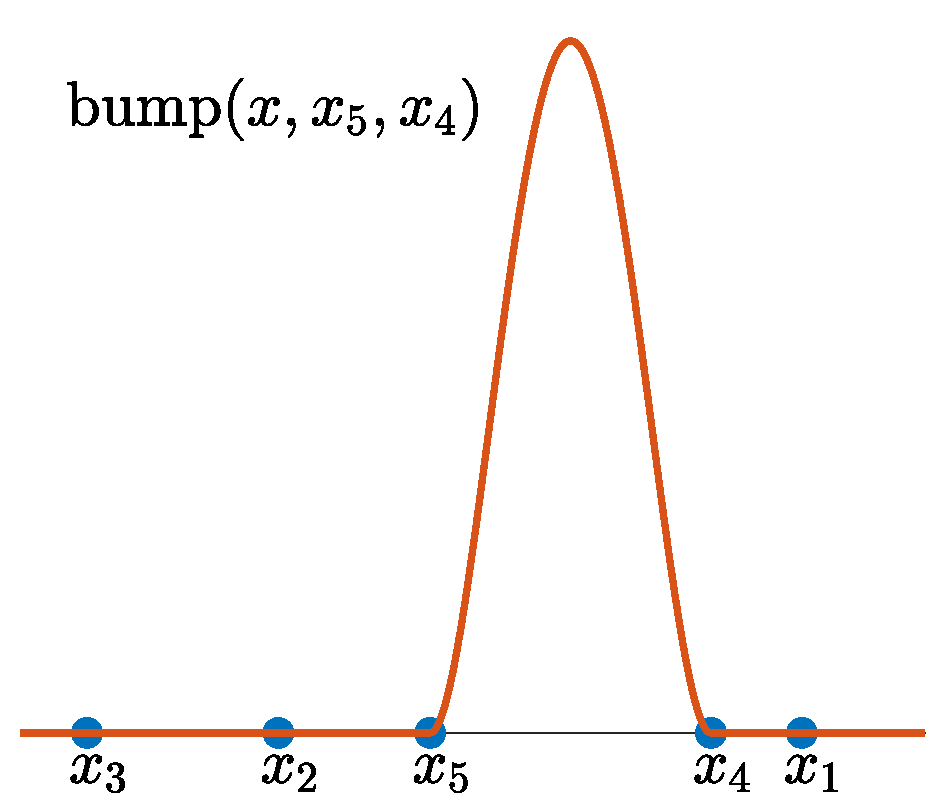
\includegraphics[height=4cm]{IntegrationBump.eps}
	\end{textblock}
	
	
\end{frame}

\begin{frame}[label = difference]{What Makes the Difference?}
	
	\vspace{-4ex}
Why
\begin{itemize}
	\item Does a trapezoidal rule algorithm exist for \hyperlink{traprule}{\beamergotobutton{this integration problem}} \\[2ex]
	
	\uncover<3->{No arbitrarily peaky functions are allowed because the second derivative is bounded, $\cf = \{f \in C^1[0,1] : \norm[2]{f''} \le \alert{1}\}$.  $\cf$ is a \alert{ball}.}\\[4ex]
	
	\item But no algorithm exists for  for \hyperlink{integnoalg}{\beamergotobutton{this other integration problem}}\\[2ex]
	
		\uncover<2->{Arbitrarily peaky functions are allowed because the second derivative is unbounded, $\cf = \{f \in C^1[0,1] : \norm[2]{f''} < \alert{\infty}\}$.  $\cf$ is a \alert{cone}, but not all cones of input functions hinder algorithms.}
	
\end{itemize}
	
\end{frame}


\part{Cost and Complexity}
\section{Algorithm Cost}
\begin{frame}{Dummy Frame}

\end{frame}


\section{Problem Complexity}


\part{Tractability}


\part{References}
\begin{frame}{References}
	\printbibliography
\end{frame}


\end{document}




\chapter{Various Error Criteria} \label{chap:relerror}
The error criterion in \cref{prob:findzerocont} requires that the location of one zero of the function be identified within an interval of half-width $\varepsilon$.  The true solution of $f(x) = 0$ can be written as the set $f^{-1}(0)$.  If the zero-finding algorithm outputs $x_0$, then the true error of the output is $\min_{x \in f^{-1}(0)} \abs{x-x_0}$. The absolute error criterion in \cref{prob:findzerocont} that the output, $x_0$, must satisfy can be expressed as 
\begin{equation} \label{eq:fzeroerrorcrit}
    \crit\bigl(x_0,f^{-1}(0),\varepsilon\bigr) = 
    \begin{cases} \true, & \exists x \in f^{-1}(0) \text{ such that } \abs{x-x_0} \le \varepsilon,\\
    \false, & \text{otherwise}.
    \end{cases}
\end{equation}

In practice, it is not possible to know the true error of the output, but \cref{alg:zeroBisectionAB} iteratively refines the interval $[x_{\text{left}}, x_{\text{right}}]$ that must contain at least one zero of $f$. 
The data-driven stopping criterion for \cref{alg:zeroBisectionAB} may be expressed by replacing the true solution by the all possible partial solutions as
\begin{equation}
    \datacrit\bigl(x_0,[x_{\text{left}},x_{\text{right}}],\varepsilon\bigr) = 
    \begin{cases} \true, & \crit\bigl(x_0,\{x\},\varepsilon\bigr) = \true \ \ \forall x \in [x_{\text{left}},x_{\text{right}}] ,\\
    \false, & \text{otherwise},
    \end{cases}
\end{equation}

Choosing $x_0 = (x_{\text{left}}+x_{\text{right}})/2$ as is done in \cref{alg:zeroBisectionAB} gives the stopping criterion the best chance of being $\true$.  When $\datacrit\bigl(x_0,[x_{\text{left}},x_{\text{right}}],\varepsilon\bigr) = \true$, then \cref{alg:zeroBisectionAB} stops and returns $x_0$.

In some cases, the practitioner may wish to choose a different kind of error criterion than an absolute one, such as a relative error criterion or one involving a combination of absolute and relative error tolerances.  In such cases, choosing the middle of the interval containing the solution may be not be best.  In this chapter we explore various error criteria, their corresponding stopping criteria, and the choices of outputs.

\section{A Generic Numerical Problem and Template Algorithm}

Let's generalize the zero-finding situation to a generic numerical problem.  As before, we let $\cf$ denote the set of input functions, which must be large enough so that the successful algorithm is widely applicable but constrained so that a successful algorithm exists. 

\begin{NumProblem}[Generic Numerical Problem]
\label{prob:generalProblem}
\problemspecs{set of functions $\cf$ \\ 
solution operator $\sol: \cf \to \cg$}
{black-box function $f \in \cf$ \\ error tolerance (vector) $\veps$}
{$\out \in \ca$ such that \\ \qquad $\crit(\out,\sol(f),\veps) = \true$}
\end{NumProblem}

The solution operator, $\sol$, maps an element in $\cf$ to a \emph{set} of acceptable solutions, not a single solution. This is to allow for the case of non-unique acceptable solutions. For example, if $f: x \mapsto x^3 - x$ defined on $[-2,2]$, then $\sol(f) = \{-1, 0, 1\}$ for zero-finding \cref{prob:findzerocont}, where only one zero is required, but  $\sol(f) = \{ \{-1, 0, 1\} \}$ for \cref{prob:findzerocontall}, where all zeros are required.  The set of sets of acceptable solutions is denoted $\cg$.

The output required from the problem comes from the set of acceptable solutions $\ca$.  The elements of $\ca$ are the elements of the elements of $\cg$, i.e., $\ca = \{S \in G : G \in \cg\}$.  For $f: x \mapsto x^3 - x$ defined on $[-2,2]$ in zero-finding \cref{prob:findzerocont}, $\out$ is a number sufficiently close to $-1$ or $0$ or $1$.  For \cref{prob:findzerocontall}, $\out$ for this same function is a set sufficiently close to  $\{-1, 0, 1\}$.  The sets $\cf$, $\cg$, and $\ca$ are tabulated for different problems in \cref{tab:genericproblem}.  

\begin{table}[H]
    \centering
    \caption{Examples of specific problems following Generic \cref{prob:generalProblem}}
      {\small \begin{tabular}{c>{\centering}m{0.21\textwidth}>{\centering}m{0.15\textwidth}>{\centering}m{0.25\textwidth}>{\centering}m{0.2\textwidth}}
       \multicolumn{2}{c}{Problem} & Inputs, $\cf$ & $\cg$ & $\ca$
         \tabularnewline \toprule
         \ref{prob:findzerocont} & 
         $\sol(f) = f^{-1}(0)$ & $\bigcup_{a < b} C[a,b]$ \\ $f(a)f(b) \le 0$ & closed, bounded subsets of $\reals$ & $\reals$
        \tabularnewline \midrule
        \ref{prob:findzerocontall} &
        $\sol(f) = \{f^{-1}(0)\}$ & $\bigcup_{a < b} C[a,b]$ & sets with a single element: a closed, bounded subset of $\reals$  & 
        closed, bounded subsets of $\reals$
        \tabularnewline \bottomrule
        \end{tabular} }
    \label{tab:genericproblem}
\end{table}

The error criterion, $\crit: \ca \times \cg \times (0,\infty)^s \to \{\true, \false\}$, specifies how close the output must be to an element in $\sol(f)$.  The first input is an algorithm output, the second input is the true solution, and the third input is a (vector) error tolerance.  The error criterion for the zero-finding problem defined in \eqref{eq:fzeroerrorcrit} is an example.  Various error criteria are discussed in this chapter.

Next we define a template \cref{alg:template} for \cref{prob:generalProblem}.  The algorithm works with $\cs$, a set of acceptable solutions consistent with the function data.  We initialize $\cs$ to be $\ca$, the whole set of acceptable solutions, which is also are set of possible outputs.
At each iteration, the algorithm samples $f$ further and shrinks $\cs$ to be consistent with all function data.  A data-based stopping criterion is defined by determining whether the error criterion for the problem is true for all possible acceptable solutions in $\cs$:
\begin{equation}
    \datacrit(\out,\cs,\veps) = \begin{cases} \true, & \crit(\out,S,\veps) = \true \quad \forall S \in \cs, \\ \false, & \text{otherwise} .
    \end{cases}
\end{equation}
When $\cs$ becomes small enough so that an output exists that $\out$ exists that makes the stopping criterion $\true$, then the algorithm terminates.

\begin{algorithm}[H]
\caption{Template algorithm for Generic Numerical \cref{prob:generalProblem} \label{alg:template}}
	\begin{algorithmic}
   \State Initialize $\cs$, the set containing acceptable solutions consistent with function data, to be $\ca$
   \State Shrink $\cs$ based on an initial sample of $f$
    \Repeat 
    \State Shrink $\cs$ further based on further sampling of $f$
    \State Choose $\out$ optimally
    \Until $\datacrit(\out,\cs,\varepsilon) = \true$
    \RETURN $\out$
    \end{algorithmic}
\end{algorithm}



\section{Absolute Error Criterion} \label{sec:abserror}
The error criterion for the zero-finding problem defined in \eqref{eq:fzeroerrorcrit}  is an absolute error criterion, which requires that the output be within $\varepsilon$ of the true answer. The following is a more general absolute error criterion where the set of acceptable solutions, $\ca$, is a subset of the real numbers: 
\begin{equation} \label{eq:absnormerrorcrit}
    \crit(\out,\sol(f),\varepsilon) = 
    \begin{cases} \true, & \exists S \in \sol(f) \text{ with } \abs{\out-S} \le \varepsilon,\\
    \false, & \text{otherwise}.
    \end{cases}
\end{equation}

For the If $\cs$, the set of acceptable solutions consistent with the function data in \cref{alg:template}, is the interval $\cs = [S_{\lo}, S_{\high}]$, then the optimal choice of $\out$ is the center of the interval.

\cref{tab:errorcrit} shows the optimal choices of the output, $\out$ for various error criteria that can be expressed in terms of the absolute value between the output and the solution and where an acceptable true solution is known to be in $[S_{\lo}, S_{\high}]$.  In the following sections we explore relative and compound error criteria.  In these cases, the interval midpoint may not be the optimal choice for $\out$.


\begin{table}[H]
    \centering
    \caption{Conditions under which the error criterion is true and the corresponding optimal output when an acceptable true solution lies in $\cs = [S_{\lo}, S_{\high}]$.}
    \begin{equation*}
       \begin{array}{ccc}
         \crit(\out,\sol(f),\varepsilon) && \text{Sufficient condition for}\\
         \exists S \in \sol(f) \text{ such that}
         & \out 
         & \datacrit(\out,\cs,\varepsilon) = \true \tabularnewline \toprule
        \abs{\out-S} \le \varepsilon & 
        (S_{\lo} + S_{\high})/2 &
        S_{\high} - S_{\lo} < 2\varepsilon \\
         \midrule
         \abs{\out-S} \le \varepsilon \abs{G} 
         & 
        \end{array} 
    \end{equation*}
    
    \label{tab:errorcrit}
\end{table}

\section{Relative Error}
Sometimes the error requirement is relative to the size of the answer, e.g., 
\begin{equation} \label{eq:absnormerrorcrit}
    \crit(\out,\sol(f),\varepsilon) = 
    \begin{cases} \true, & \exists S \in \sol(f) \text{ with } \abs{\out-S} \le \varepsilon \abs{S},\\
    \false, & \text{otherwise}.
    \end{cases}
\end{equation}
Here we assume that the relative error tolerance, $\varepsilon$. is strictly less than one.
The relative error criterion in \eqref{eq:absnormerrorcrit} is true if
\begin{equation}
    \min_{\out \in \ca} g(\out) \le 0, \quad \text{where } g(t) = \max_{S_{\lo} \le S \le S_{\high}} h(t,S), \quad h(t,S) = \abs{t - S} - \varepsilon \abs{S},
\end{equation}
where the set of solutions consistent with the function data is $[S_{\lo}, S_{\high}]$.
Note that it is impossible to satisfy this sufficient condition if $S_{\lo}S_{\high} \le 0$.

The function $h(t,\cdot)$ is piecewise linear with a slope corresponding to $\sign(\cdot-t)$ since $\varepsilon < 1$.  Thus, $h(t,\cdot)$ obtains its maximum at $S_{\lo}$ or $S_{\high}$, i.e., $g(t)$ corresponds to $h(t,S_{\lo})$ or $h(t,S_{\high})$.  The functions $h(\cdot,S_{\lo})$ and $h(\cdot,S_{\high})$ are also piececwise linear.  Thus, the value of $t$ that  minimizes $g(t)$ is the one for which $h(t,S_{\lo}) = h(t,S_{\high})$.  This optimal value of $\out$ satisfies
\begin{gather*}
    \abs{\out - S_{\lo}} - \varepsilon \abs{S_{\lo}} = \abs{\out - S_{\high}} - \varepsilon \abs{S_{\high}}
\end{gather*}